\section{具有某些特性的函数}

\subsection{有界函数}

\begin{definition}[有界函数]
    设 $f$ 为定义在 $D$ 上的函数.若存在数 $M(L)$,使得对每一个 $x\in D$,都有 $f(x)\le M (f(x)\ge L)$,则称 $f$ 为 $D$ 上的\textbf{有上(下)界函数},$M(L)$ 称为 $f$ 在 $D$ 上的一个\textbf{上(下)界}.
\end{definition}

根据定义,$f$ 在 $D$ 上有上(下)界,意味着值域 $f(D)$ 是一个有上(下)界的数集.又若 $M(L)$ 为 $f$ 在 $D$ 上的上(下)界,则任何大于(小于)$M(L)$ 的数也是 $f$ 在 $D$ 上的上(下)界.

\begin{definition}
    设 $f$ 为定义在 $D$ 上的函数.若存在正数 $M$,使得对每一个$x\in D$,有 $\abs{f(x)}\le M$,则称 $f$ 为 $D$ 上的 \textbf{有界函数}.
\end{definition}

根据定义,$f$ 在 $D$ 上有界,意味着值域 $f(D)$ 是一个有界集.又按定义,不难验证:$f$ 在 $D$ 上有界的充要条件是 $f$ 在 $D$ 上既有上界又有下界.同时,从几何意义上看,$f$ 在 $D$ 上有界,那么 $f$ 的图像将完全落在直线 $y=M$ 和 $y=-M$ 之间.

例如,正弦函数 $\sin x$ 和余弦函数 $\cos x$ 为 $\R$ 上的有界函数,因为对每一个$x\in \R$,都有 $\abs{\sin x}\le 1$ 和 $\abs{\cos x}\le 1$.

关于函数 $f$ 在数集 $D$ 上无上界、无下界或无界的定义,可按上述相应定义的否定说法来叙述.例如,设$f$ 为定义在 $D$ 上的函数,若对任何 $M$ (无论 $M$ 多大),都存在 $x_0\in D$,使得 $f(x_0)>M$,则称 $f$ 为 $D$ 上的\textbf{无上界函数}.

作为练习,读者可以自行写出无下界函数与无界函数的定义.

\begin{example}
    证明 $f(x)=\frac{1}{x}$ 为 $(0,1]$ 上的无上界函数.
\end{example}

\begin{proof}
    对于任何正数 $M$,取$(0,1]$ 上的一点 $x_0=\frac{1}{M+1}$,则有 $f(x_0)=\frac{1}{x_0}=M+1>M$.
\end{proof}

前面已经指出,$f$ 在其定义域 $D$ 上有上界,是指值域$f(D)$为有上界的数集.于是由确界原理,数集 $f(D)$ 有上确界.通常,我们把 $f(D)$ 的上确界记为 $\sup_{x\in D} f(x)$,并称之为 $f$ 在 $D$上的上确界.类似地,若 $f$ 在其定义域 $D$ 上有下界,则$f$ 在 $D$上的下确界记为 $\inf_{x\in D} f(x)$.

\begin{example}\label{ex:supfx}
    设 $f,g$ 为 $D$ 上的有界函数.证明:

    (1) $\inf_{x\in D} f(x)+\inf_{x\in D} g(x)\le \inf_{x\in D} \{f(x)+g(x)\}$

    (2) $\sup_{x\in D} f(x)+\sup_{x\in D} g(x)\ge \sup_{x\in D} \{f(x)+g(x)\}$
\end{example}

\begin{proof}
    (1) 对任何 $x\in D$,都有 $\inf_{x\in D} f(x)\le f(x),\inf_{x\in D} g(x)\le g(x)$.由此可得 $\inf_{x\in D} f(x)+\inf_{x\in D} g(x)\le f(x)+g(x)$. 这说明 $\inf_{x\in D} f(x)+\inf_{x\in D} g(x)$ 是 $f(x)+g(x)$ 的一个下界,故 $\inf_{x\in D} f(x)+\inf_{x\in D} g(x)\le \inf_{x\in D} \{f(x)+g(x)\}$

    (2) 可类似证明.
\end{proof}

\begin{annotation}
    \exref{ex:supfx} 中的两个不等式,其严格的不等号有可能成立.例如,设 $f(x)=x,g(x)=-x,x\in [-1,1]$,则有 $\inf_{\abs{x}<1} f(x)=\inf_{\abs{x}<1} g(x)=-1$,$\sup_{\abs{x}<1} f(x)=\sup_{\abs{x}<1} g(x)=1$,然而 $\inf_{x\in D} \{f(x)+g(x)\}=\sup_{x\in D} \{f(x)+g(x)\}=0$
\end{annotation}

\subsection{单调函数}

\begin{definition}[单调函数]
    设 $f$ 为定义在 $D$ 上的函数.若对任何 $x_1,x_2\in D$,当 $x_1<x_2$时,总有

    (1) $f(x_1)\le f(x_2)$,则称 $f$ 为 $D$ 上的\textbf{(递)增函数},特别当成立严格不等式 $f(x_1)<f(x_2)$时,称 $f$ 为 $D$ 上的\textbf{严格(递)增函数}

    (2) $f(x_1)\ge f(x_2)$,则称 $f$ 为 $D$ 上的\textbf{(递)减函数},特别当成立严格不等式 $f(x_1)>f(x_2)$时,称 $f$ 为 $D$ 上的\textbf{严格(递)减函数}

    增函数和减函数统称为 \textbf{单调函数}.严格增函数和严格减函数统称为 \textbf{严格单调函数}.
\end{definition}

\begin{example}
    函数 $y=x^3$ 在 $\R$ 上是严格增的.因为对任何的 $x_1,x_2\in \R$,当 $x_1<x_2$ 时,总有 $x_2^3-x_1^3=(x_2-x_1)(x_2^2+x_1x_2+x_1^2)=(x_2-x_1)[(x_2+\frac{x_1}{2})^2+\frac{3}{4}x_1^2]>0$,即 $x_1^3<x_2^3$.
\end{example}

\begin{example}
    函数 $y=\lfloor x \rfloor$在 $\R$ 上是增的.因为对任何的$x_1,x_2\in \R$, 当 $x_1<x_2$ 时,显然有 $\lfloor x_1 \rfloor < \lfloor x_2 \rfloor$.但此函数在 $\R$ 上不是严格增的,若取 $x_1=0,x_2=\frac{1}{2}$  ,则有 $\lfloor x_1 \rfloor = \lfloor x_2 \rfloor = 0$,即定义中所要求的严格不等式不成立.此函数的图像如\figref{fig:floorfx}所示.
\end{example}

\begin{figure}[htbp]
    \centering
    \begin{tikzpicture}
        \draw[->,below] (-4,0)--(4,0) node {$x$};
        \draw[->,right] (0,-4)--(0,4) node {$y$};
        \foreach \x in {-2,-1,0,1,2,3}{
        \draw[red] (\x,\x-1) circle(2pt)  ;
        \draw[blue] (\x-1,\x-1)--(\x,\x-1);
        \draw[right] node at (0,\x) {$\x$};
        }
        \draw[right] node at (0,-3) {$-3$};
        \foreach \x in {1,2,3}
        \draw[below] node at (\x,0) {$\x$};
        \foreach \x in {-1,-2,-3}
        \draw[above] node at (\x,0) {$\x$};
    \end{tikzpicture}
    \caption{$y=\lfloor x \rfloor$的图像}
    \label{fig:floorfx}
\end{figure}

严格单调函数的图像与任一平行于 $x$ 轴的直线至多有一个交点,这一特性保证了它必定具有反函数.

\begin{theorem}\label{thm:zeng}
    设 $y=f(x),x\in D$ 为严格增(减)函数,则 $f$ 必有反函数 $f^{-1}$,且 $f^{-1}$ 在其定义域 $f(D)$上也是严格增(减)函数.
\end{theorem}

\begin{proof}
    设 $f$ 在 $D$ 上严格增.对任何一个 $y\in f(D)$,有 $x\in D$ 使 $f(x)=y$. 下面证明:这样的 $x$ 只能有一个.事实上,对于 $D$ 中任何一个 $x_1\ne x$,由 $f$ 在 $D$ 上的严格增性,当 $x_1<x$ 时, $f(x_1)<y$, 当 $x_1>x$ 时,有 $f(x_1)>y$,总之 $f(x_1)\ne y$. 这就说明,对每一个 $y\in f(D)$,都只存在唯一的一个 $x\in D$,使得 $f(x)=y$,从而函数 $f$ 存在反函数 $x=f^{-1}(y),y\in f(D)$.

    现证 $f^{-1}$ 也是严格增的.任取 $y_1,y_2\in f(D),y_1<y_2$. 设 $x_1=f^{-1}(y_1),x_2=f^{-2}(y_2)$,则 $y_1=f(x_1),y_2=f(x_2)$.由 $y_1<y_2$ 及 $f$ 的单调性,显然有 $x_1<x_2$,即 $f^{-1}(y_1)<f^{-1}(y_2)$.所以反函数 $f^{-1}$ 是严格增的.
\end{proof}

\begin{example}
    函数 $y=x^2$ 在 $[0,+\infty)$ 是严格增的,其值域为 $[0,+\infty)$,故有反函数 $y=\sqrt{x},x\in [0,+\infty)$;函数 $y=x^2$ 在 $(-\infty,0)$ 是严格减的,其值域为 $(0,+\infty)$,故有反函数 $y=-\sqrt{x},x\in (0,+\infty)$. 但 $y=x^2$ 在整个定义域 $\R$ 上不是单调的,也不存在反函数.
\end{example}

上节中我们给出了实指数幂的定义,从而将指数函数 $y=a^x(a>0,a\ne 1)$ 的定义域拓广到整个实数集 $\R$. 下面证明指数函数在 $\R$ 上的严格单调性.

\begin{example}\label{ex:ax}
    证明: $y=a^x$ 当 $a>1$ 时在在 $\R$ 上严格递增,当 $0<a<1$ 时在 $\R$ 上严格递减.
\end{example}

\begin{proof}
    设 $a>1$ . 给定 $x_1,x_2\in \R,x_1<x_2$.由有理数集的稠密性,可取到有理数 $r_1,r_2$,使得 $x_1<r_1<r_2<x_2$(参见\exref{ex:inside}),故有 $a^{x_1} = \sup_{r\le x_1}\setset{a^r}{r\mbox{为有理数}} \le a^{r_1}<a^{r_2}\le \sup_{r\le x_2}\setset{a^r}{r\mbox{为有理数}}=a^{x_2}$,这就证明了 $y=a^x$ 当 $a>1$ 时在在 $\R$ 上严格递增.

    类似地可以证明$y=a^x$ 当 $0<a<1$ 时在 $\R$ 上严格递减.
\end{proof}

\begin{annotation}
    因为 $y=a^x(a>0,a\ne 1)$ 的值域为 $(0,+\infty)$, 所以由\exref{ex:ax}及\thmref{thm:zeng}还可得出结论:对数函数 $y=\log_a x$ 当 $a>1$ 时在 $(0,+\infty)$ 上严格递增,当 $0<a<1$ 时在 $(0,+\infty)$ 上严格递减.另外,在第四章中将证明关于实指数幂的一个基本性质$(a^\alpha)^\beta=a^{\alpha\beta}$,从而相应地有 $\log_a x^\alpha = \alpha \log_a x(a>0,a\ne 1,x\in\R^+,\alpha \in \R)$.
\end{annotation}

\subsection{奇函数与偶函数}

\begin{definition}[函数的奇偶性]
    设 $D$ 为对称于原点的数集, $f$ 为定义在 $D$ 上的函数. 若对每一个 $x\in D$ ,有 $f(-x)=-f(x)$ ,则称 $f$ 为 $D$ 上的\textbf{奇函数}.若对每一个 $x\in D$ ,有 $f(-x)=f(x)$ ,则称 $f$ 为 $D$ 上的\textbf{偶函数}.
\end{definition}

从函数图形上来看,奇函数的图像关于原点对称,偶函数的图像则关于 $y$ 轴对称.

例如,正弦函数 $y=\sin x$ 和正切函数 $y=\tan x$ 是奇函数,余弦函数 $y=\cos x$ 是偶函数,符号函数是奇函数. 而函数 $f(x)=\sin x+\cos x$ 既不是奇函数,也不是偶函数.因为如果取 $x_0=\frac{\pi}{4}$, 则 $f(x_0)=\sqrt{2},f(-x_0)=0$,显然既不成立 $f(-x_0)=-f(x_0)$, 也不成立 $f(-x_0)=f(x_0)$.

\subsection{周期函数}

\begin{definition}[周期函数]
    设 $f$ 为定义在数集 $D$ 上的函数.若存在 $\sigma>0$,使得对一切 $x\in D$,有 $x\pm \sigma \in D$,且 $f(x\pm \sigma)=f(x)$,则称 $f$ 为\textbf{周期函数},$\sigma$ 为 $f$ 的一个\textbf{周期}.显然,若 $\sigma$ 为 $f$ 的周期, 则 $n\sigma$ ($n$ 为正整数)也是 $f$ 的周期.若在周期函数 $f$ 的所有周期中有一个最小的周期,则称此最小周期为 $f$ 的\textbf{基本周期},或简称\textbf{周期}.
\end{definition}
例如,$\sin x$ 的周期为 $2\pi$,$\tan x$ 的周期为 $\pi$,函数 $f(x)=x-\lfloor x \rfloor,x\in \R$ 的周期为 1(\figref{fig:xfloorfx}),常量函数 $f(x)=c$ 是以任何正数为周期的周期函数,但不存在基本周期.

\begin{figure}[htbp]
    \centering
    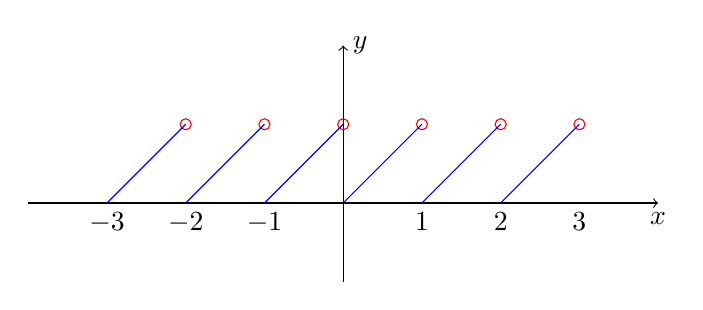
\begin{tikzpicture}
        \draw[->,below] (-4,0)--(4,0) node {$x$};
        \draw[->,right] (0,-1)--(0,2) node {$y$};
        \foreach \x in {-2,-1,0,1,2,3}{
        \draw[red] (\x,1) circle(2pt)  ;
        \draw[blue] (\x-1,0)--(\x,1);
        }
        \foreach \x in {1,2,3}
        \draw[below] node at (\x,0) {$\x$};
        \foreach \x in {-1,-2,-3}
        \draw[below] node at (\x,0) {$\x$};
    \end{tikzpicture}
    \caption{$y=x - \lfloor x \rfloor$的图像}
    \label{fig:xfloorfx}
\end{figure}

\homework

\begin{practice}
    证明 $f(x)=\frac{x}{x^2+1}$ 是 $\R$ 上的有界函数.
\end{practice}

\begin{proof}
    对于任意的 $x\in \R$ ,若 $x\ne 0$ ,则$\abs{\frac{x}{x^2+1}}=\frac{\abs{x}}{(\abs{x})^2+1}<\frac{1}{\abs{x}+\frac{1}{\abs{x}}}\le \frac{1}{2}$;若 $x=0$,也有$\abs{\frac{x}{x^2+1}}=0<\frac{1}{2}$,故 $M=\frac{1}{2}$ 是 $f$ 的一个界.
\end{proof}

\begin{practice}
    (1) 叙述无界函数的定义

    (2) 证明 $f(x)=\frac{1}{x^2}$ 为 $(0,1)$ 上的无界函数.

    (3) 举出 $f$ 的例子,使 $f$ 为闭区间 $[0,1]$ 上的无界函数.
\end{practice}

\begin{solve}
    (1) 设 $f$ 为定义在 $D$ 上的函数.若对任意的正数 $M$,都存在着$x_0\in D$,有 $\abs{f(x)}> M$,则称 $f$ 为 $D$ 上的无界函数.

    (2) 对任意的正数 $M$,都存在着$x_0=\frac{1}{\sqrt{M+1}}\in (0,1)$,有 $\abs{\frac{1}{x_0^2}}=M+1> M$,故 $f$ 为 $D$ 上的无界函数.

    (3) 如 $f(x)=\begin{cases}
        0 & x=0 \\ 
        \frac{1}{x^2} & 0<x\le 1
    \end{cases}$
\end{solve}

\begin{practice}
    证明下列函数在指定区间上的单调性:

    (1) $y=3x-1$ 在 $(-\infty,\infty)$ 上严格递增.

    (2) $y=\sin x$ 在 $[-\frac{\pi}{2},\frac{\pi}{2}]$ 上严格递增.

    (3) $y=\cos x$ 在 $[0,\pi]$ 上严格递减.
\end{practice}

\begin{proof}
    (1) 任意 $x_1<x_2\in (-\infty,\infty)$,有 $y_1-y_2=(3x_1-1)-(3x_2-1)=3(x_1-x_2)<0$,即 $y_1<y_2$,故$y=3x-1$ 在 $(-\infty,\infty)$ 上严格递增.

    (2) 任意 $x_1<x_2\in [-\frac{\pi}{2},\frac{\pi}{2}]$,有 $y_1-y_2=\sin x_1-\sin x_2=\sin (\frac{x_1+x_2}{2}+\frac{x_1-x_2}{2})+\sin (\frac{x_1+x_2}{2}-\frac{x_1-x_2}{2})=2 \cos \frac{x_1+x_2}{2}\sin \frac{x_1-x_2}{2}$.
    
    $\frac{x_1+x_2}{2}\in (-\frac{\pi}{2},\frac{\pi}{2})$,故 $\cos \frac{x_1+x_2}{2}>0$. $\frac{x_1-x_2}{2}\in [-\frac{\pi}{2},0)$,故 $\sin \frac{x_1-x_2}{2}<0$. 

    则 $y_1<y_2$.故$y=\sin x$ 在 $[-\frac{\pi}{2},\frac{\pi}{2}]$ 上严格递增.
    
    (3) 任意 $x_1<x_2\in [0,\pi]$,有 $y_1-y_2=\cos x_1-\cos x_2 = \cos (\frac{x_1+x_2}{2}+\frac{x_1-x_2}{2})+\cos (\frac{x_1+x_2}{2}-\frac{x_1-x_2}{2})=-2 \sin \frac{x_1+x_2}{2}\sin \frac{x_1-x_2}{2}$.

    $\frac{x_1+x_2}{2}\in (0,\pi)$,故 $\sin \frac{x_1+x_2}{2}>0$. $\frac{x_1-x_2}{2}\in [-\frac{\pi}{2},0)$,故 $\sin \frac{x_1-x_2}{2}<0$. 

    则 $y_1<y_2$. 故 $y=\cos x$ 在 $[0,\pi]$ 上严格递减.
\end{proof}

\begin{practice}
    判别下列函数的奇偶性:

    (1) $f(x)=\frac{1}{2} x^4 +x^2-1$ \quad (2) $f(x)=x+\sin x$

    (3) $f(x)=x^2e^{-x^2}$ \quad (4) $f(x)=\lg (x+\sqrt{1+x^2})$
\end{practice}

\begin{solve}
    (1) $f(-x)=\frac{1}{2} (-x)^4 +(-x)^2-1=\frac{1}{2} x^4 +x^2-1=f(x),x\in \R$.故 $f(x)$ 是偶函数.

    (2) $f(-x)=-x+\sin(-x)=-x-\sin x=-(x+\sin x)=-f(x),x\in \R$.故 $f(x)$ 是奇函数.

    (3) $f(-x)=(-x)^2e^{-(-x)^2}=x^2e^{-x^2}=f(x),x\in \R$.故 $f(x)$ 是偶函数.

    (4) $f(-x)=\lg (-x+\sqrt{1+(-x)^2})=-\lg \frac{1}{-x+\sqrt{1+(-x)^2}}=-\lg \frac{x+\sqrt{1+x^2}}{(x+\sqrt{1+x^2})(-x+\sqrt{1+x^2})}=-\lg \frac{x+\sqrt{1+x^2}}{(1+x^2)-x^2}=-\lg (-x+\sqrt{1+x^2})=-f(x),x\in \R$.故 $f(x)$ 是奇函数.
    
\end{solve}

\begin{practice}
    求下列周期函数的周期:

    (1)$\cos^2 x$ \qquad (2) $\tan 3x$ \qquad (3) $\cos \frac{x}{2} + 2\sin \frac{x}{3}$
\end{practice}

\begin{solve}
    (1) $\cos^2 x=\frac{1+\cos 2x}{2}$. 而 $\cos 2x$ 的周期为 $T=\frac{2\pi}{2}=\pi$. 故 $\cos^2 x$ 的周期为 $\pi$. 

    (2) $\tan x$ 的周期为 $T_0=\pi$, 故 $\tan 3x$ 的周期为 $\frac{T_0}{3}=\frac{\pi}{3}$.

    (3) $\cos \frac{x}{2}$ 的周期为 $\frac{2\pi}{\frac{1}{2}}=4\pi$. $\cos \frac{x}{3}$ 的周期为 $\frac{2\pi}{\frac{1}{3}}=6\pi$.4 与 6的最小公倍数为 12, 故 $\cos \frac{x}{2} + 2\sin \frac{x}{3}$的周期为$12\pi$.
\end{solve}

\begin{practice}
    设函数 $f$ 定义在 $[-a,a]$ 上,证明:

    (1) $F(x)=f(x)+f(-x),x\in [-a,a]$ 为偶函数

    (2) $G(x)=f(x)-f(-x),x\in [-a,a]$ 为奇函数

    (3) $f$ 可表示成某个奇函数与某个偶函数之和.
\end{practice}

\begin{proof}
    (1) $F(-x)=f(-x)+f(x)=F(x),x\in [-a,a]$. 故 $F(x)$ 为偶函数.

    (2) $G(-x)=f(-x)-f(x)=-[f(x)-f(-x)]=-G(x),x\in [-a,a]$. 故 $G(x)$ 为奇函数.

    (3) $f(x)=\frac{[f(x)+f(-x)]+[f(x)-f(-x)]}{2}=\frac{F(x)-G(x)}{2}$. $\frac{F(x)}{2}$ 为偶函数,$\frac{G(x)}{2}$ 为奇函数.
\end{proof}

\begin{practice}
    由三角函数的两角和差公式
    \[
    \sin (\alpha\pm \beta) = \sin \alpha \cos \beta \pm \sin \beta \cos \alpha
    \]
    \[
    \cos (\alpha\pm \beta) = \cos \alpha \cos \beta \mp \sin \beta \sin \alpha
    \]
    推出:
    
    (1)和差化积公式
    \[
    \sin \alpha + \sin \beta = 2\sin \frac{\alpha+\beta}{2} \cos \frac{\alpha-\beta}{2}
    \]
    \[
    \sin \alpha - \sin \beta = 2\sin \frac{\alpha-\beta}{2} \cos \frac{\alpha+\beta}{2}
    \]
    \[
    \cos \alpha + \cos \beta = 2\cos \frac{\alpha+\beta}{2} \cos \frac{\alpha-\beta}{2}
    \]
    \[
    \cos \alpha - \cos \beta = -2\sin \frac{\alpha+\beta}{2} \sin \frac{\alpha-\beta}{2}
    \]

    (2)积化和差公式
    \[
    \sin \alpha \sin \beta = \frac{1}{2}[\cos (\alpha-\beta)-\cos (\alpha+\beta)]
    \]
    \[
    \sin \alpha \cos \beta = \frac{1}{2}[\sin (\alpha+\beta)+\sin (\alpha-\beta)]
    \]
    \[
    \cos \alpha \cos \beta = \frac{1}{2}[\cos (\alpha+\beta)+\cos (\alpha-\beta)]
    \]
    \[
    \sin \alpha \sin \beta = -\frac{1}{2}[\cos (\alpha+\beta)-\cos (\alpha-\beta)]
    \]
\end{practice}

\begin{proof}
    令和差化积公式等号左边的 $\alpha=\frac{\alpha+\beta}{2}+\frac{\alpha-\beta}{2},\beta=\frac{\alpha+\beta}{2}-\frac{\alpha-\beta}{2}$,根据两角和差公式展开,即可得到和差化积公式.将两角和差公式公式进行加减数乘运算即可得到积化和差公式.
\end{proof}

\begin{practice}
    设 $f,g$ 为定义在 $D$ 上的有界函数,满足 $f(x)\le g(x),x\in D$.证明:

    (1) $\sup_{x\in D} \{f(x)\}\le \sup_{x\in D} \{g(x)\}$ \qquad
    (2) $\inf_{x\in D} \{f(x)\}\le \inf_{x\in D} \{g(x)\}$
\end{practice}

\begin{proof}
    (1) 对于任何 $x\in D$,有 $ f(x)\le g(x)\le \sup_{x\in D} \{g(x)\}$. 故 $\sup_{x\in D} \{g(x)\}$ 是 $f(x)$ 的一个上界,则 $\sup_{x\in D} \{f(x)\}\le \sup_{x\in D} \{g(x)\}$.

    (2) 对于任何 $x\in D$,有 $\inf_{x\in D} \{f(x)\}\le f(x)\le g(x)$. 故 $\inf_{x\in D} \{f(x)\}$ 是 $g(x)$ 的一个下界,则 $\inf_{x\in D} \{f(x)\}\le \inf_{x\in D} \{g(x)\}$.
\end{proof}

\begin{practice}
设 $f$ 为定义在 $D$ 上的有界函数,证明:

    (1) $\sup_{x\in D} \{-f(x)\}=-\inf_{x\in D} \{f(x)\}$ \qquad
    (1) $\inf_{x\in D} \{-f(x)\}=-\sup_{x\in D} \{f(x)\}$
\end{practice}

\begin{proof}
    (1) 记 $\xi=\inf_{x\in D} \{f(x)\}$,则在 $D$ 上 $f(x)\ge \xi$ 且 $\forall \beta>\xi,$ 都存在 $x_0$ 使得 $f(x_0)<\beta$. 也就是说,$-f(x)\le -\xi$ 且 $\forall -\beta<-\xi,$ 都存在 $x_0$ 使得 $-f(x_0)>-\beta$. 故 $-\xi$ 为 $-f(x)$ 的上确界.即 $\sup_{x\in D} \{-f(x)\}=-\inf_{x\in D} \{f(x)\}$.

    (2) 记 $\eta=\sup_{x\in D} \{f(x)\}$,则在 $D$ 上 $f(x)\le \eta$ 且 $\forall \alpha<\eta,$ 都存在 $x_0$ 使得 $f(x_0)>\alpha$. 也就是说,$-f(x)\ge -\eta$ 且 $\forall -\alpha>-\eta,$ 都存在 $x_0$ 使得 $-f(x_0)<-\alpha$. 故 $-\eta$ 为 $-f(x)$ 的下确界.即 $\inf_{x\in D} \{-f(x)\}=-\sup_{x\in D} \{f(x)\}$.
\end{proof}

\begin{practice}
    证明: $\tan x$ 在 $(-\frac{\pi}{2},\frac{\pi}{2})$ 上无界,而在任何一个闭区间 $[a,b]\subset (-\frac{\pi}{2},\frac{\pi}{2})$ 上有界.
\end{practice}

\begin{proof}
    对于任意的 $M>0$,存在 $x_0=\arctan (M+1)\in (-\frac{\pi}{2},\frac{\pi}{2})$,使得 $|\tan x_0|=M+1>M$,故$\tan x$ 在 $(-\frac{\pi}{2},\frac{\pi}{2})$ 上无界.

    存在 $M=\max \{\abs{\tan a},\abs{\tan b}\}$,使得对任意的 $x\in [a,b]\subset (-\frac{\pi}{2},\frac{\pi}{2})$, 都有 $|\tan x|\le 
    M$. 
\end{proof}

\begin{practice}
    讨论狄利克雷函数\[
D(x) = \begin{cases}
    1,& \mbox{当} x \mbox{为有理数} \\ 
    0,& \mbox{当} x \mbox{为无理数}
\end{cases}
\]的有界性、单调性与周期性.
\end{practice}

\begin{solve}
    存在 $M=1$,使得 $\forall x\in \R$, 有 $\abs{D(x)}=0\mbox{\ 或\ }1\le M$,故 $D(x)$ 为有界函数.

    取 $x_1$ 为有理数,则存在无理数 $x_2>x_1$, 使得 $D(x_2)=0\le 1=D(x_1)$. 取 $x_1$ 为无理数, 则存在有理数 $x_2>x_1$, 使得 $D(x_2)=1\ge 0=D(x_1)$. 故 $D(x)$ 无单调性.

    由于\ 有理数+有理数=有理数,无理数+有理数=无理数,所以对任意的 $x\in \R,T\in \mathbb{Q}$ ,有 $D(x+T)=D(x)$. 即任意有理数都是狄利克雷函数的周期.但狄利克雷函数没有基本周期.
\end{solve}

\begin{practice}
    证明:$f(x)=x+\sin x$ 在 $\R$ 上严格递增.
\end{practice}

\begin{proof}
    任意的 $x_1<x_2$,有 $f(x_1)-f(x_2)=(x_1-x_2)+(\sin x_1 - \sin x_2)$\\ $=(x_1-x_2)-2\sin\frac{x_1-x_2}{2}\cos\frac{x_1+x_2}{2}\le (x_1-x_2)+2|\sin\frac{x_1-x_2}{2}||\cos\frac{x_1+x_2}{2}|$ \\
    $< (x_1-x_2)+2|\frac{x_1-x_2}{2}||\cos\frac{x_1+x_2}{2}|=(x_1-x_2)-2\times \frac{x_1-x_2}{2}|\cos\frac{x_1+x_2}{2}|$\\$=(x_1-x_2)(1-|\cos\frac{x_1+x_2}{2}|)\le 0. $ 即 $f(x_1)-f(x_2)<0$. 故:$f(x)=x+\sin x$ 在 $\R$ 上严格递增.
\end{proof}

\begin{practice}
    设定义在 $[a,+\infty)$ 上的函数 $f$ 在任何闭区间 $[a,b]$ 上有界. 定义$[a,+\infty)$ 上的函数 
    
    $m(x)=\inf_{a\le y \le x} f(y),M(x)=\sup_{a\le y \le x} f(y)$.试讨论 $m(x)$ 与 $M(x)$ 的图像,其中

    (1) $f(x)=\cos x,x\in [0,+\infty)$
    \qquad
    (2) $f(x)=x^2,x\in [-1,+\infty)$
\end{practice}

\begin{solve}
    在 $[a,x]$ 上 $\{f(y)\}$ 为有界数集,故 $m(x)$ 为最小值,$M(x)$ 为最大值.根据两个函数的性质,可绘制图像如下:

    \begin{figure}[htbp]
        \centering
            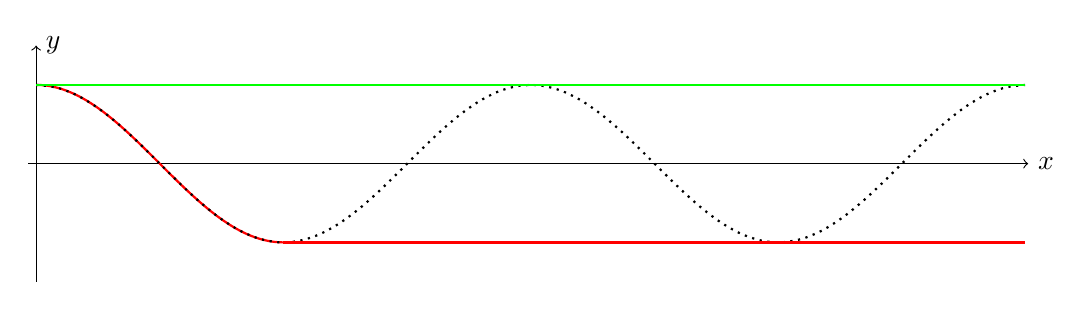
\begin{tikzpicture}
                \draw[->] (-0.1,0)--(12.6,0) node[right] {$x$};
                \draw[->] (0,-1.5)--(0,1.5) node[right] {$y$};
                \draw[red,smooth,thick,samples=50,domain=0:3.14] plot(\x,{cos(\x r)});
                \draw[dotted,smooth,thick,samples=50,domain=0:12.56] plot(\x,{cos(\x r)});
                \draw[green,smooth,thick,samples=50,domain=0:12.56] plot(\x,{1});
                \draw[red,smooth,thick,samples=50,domain=3.14:12.56] plot(\x,{-1});
            \end{tikzpicture}
            
            \begin{tikzpicture}
                \draw[->] (-1.5,0)--(2,0) node[right] {$x$};
                \draw[->] (0,-0.2)--(0,4) node[right] {$y$};
                
                \draw[green,smooth,thick,samples=50,domain=1:2] plot(\x,\x*\x);
                \draw[red,smooth,thick,samples=50,domain=-1:0] plot(\x,\x*\x);
                \draw[dotted,smooth,thick,samples=50,domain=-1:2] plot(\x,\x*\x);
                \draw[green,smooth,thick,samples=50,domain=-1:1] plot(\x,1);
                \draw[red,smooth,thick,samples=50,domain=0:2] plot(\x,0);
            \end{tikzpicture}
    \end{figure}
\end{solve}